% vim: tw=80 sw=2 ts=2 ff=unix spelllang=en spell
\documentclass{beamer}
\newcommand{\colA}[1]{\begin{columns}[t]\begin{column}{#1}}
\newcommand{\colB}[1]{\end{column}\begin{column}{#1}}
\newcommand{\colEnd}{\end{column}\end{columns}}

\usetheme{CambridgeUS}
\usecolortheme{dolphin}
%\setbeamercovered{transparent}
%\useoutertheme{infolines}

\usepackage{xltxtra}
\usepackage{fancyvrb}
%% \usepackage{ngerman}
\institute[]{Centrum für Informations- und Sprachverarbeitung (CIS)\\
            Ludwig-Maximilians-Universität München (LMU)\\
            \vspace{1cm}
            \href{https://creativecommons.org/licenses/by-nc-sa/4.0/}%
            {\includegraphics[width=0.2\textwidth]{../presentations/images/by-nc-sa.eps}}}

% keine Navigationspfeile
\setbeamertemplate{navigation symbols}{} % keine Navigations-Buttons

% Standardschrift verändern für Griechisch
%\setsansfont[Mapping=tex-text]{Junicode}
%\setmonofont[Mapping=tex-text]{DejaVu Sans Mono}
%\setsansfont[Mapping=tex-text]{Linux Libertine O}
%\setsansfont[Scale=MatchLowercase]{Linux Biolinum O}

% Fußzeile mit Titel und Seitenr.
\definecolor{mygray}{gray}{0.25}
%\setbeamertemplate{footline}[frame number]
\setbeamertemplate{footline}{\color{mygray}\hspace*{2mm}\insertauthor\hfill \insertshorttitle\hfill\insertdate\hspace*{10pt}\insertframenumber\ / \inserttotalframenumber\hspace*{2ex}}

% Schrift für URLs
\definecolor{myblue}{rgb}{0.2 0.0 0.8}

\usepackage{hyperref}
\renewcommand{\UrlFont}{\color{myblue}\footnotesize\sf}
\hypersetup{colorlinks,allcolors=.,urlcolor=blue}

% Bibliography
%\usepackage[backend=biber,style=authoryear,maxcitenames=2,maxbibnames=9]{biblatex}

% Schriftgröße Listings
\RequirePackage{fancyvrb}
\DefineVerbatimEnvironment{Highlighting}{Verbatim}%
  {commandchars=\\\{\},fontsize=\footnotesize}
\DefineVerbatimEnvironment{Verbatim}{Verbatim}%
  {fontsize=\footnotesize}
\newcommand{\pocoto}{\texttt{PoCoTo}}

\title{DATeCH 2017 -- \pocoto{} Workshop -- Introduction}
\author{Florian~Fink \& Uwe~Springmann}
%% {
%% 	Florian~Fink \href{mailto:finkf@cis.lmu.de}{finkf@cis.lmu.de}\\
%% 	Uwe~Springmann
%% 	\href{mailto:uwe.springmann@uni-wuerzburg.de}{uwe.springmann@uni-wuerzburg.de}
%% }

\begin{document}

\begin{frame}
	\titlepage
\end{frame}

\section{Introduction}
\subsection{Schedule}
\begin{frame}
	\begin{itemize}
		\item 13:00 - 13:15: Introduction
		\item 13:15 - 14:00: \pocoto{}
		\item 14:00 - 15:00: Hands on \pocoto{}
		\item 15:00 - 15:30: Profiler
		\item 15:30 - 16:00: Coffee break
		\item 16:00 - 17:00: Hands on Profiler
	\end{itemize}
\end{frame}

\subsection{Overview}
\begin{frame}
	This Workshop covers two main topics:
	\begin{enumerate}
		\item The \pocoto{} PostCorrectionTool: A tool to do interactive
			postcorrection of OCR'ed (historical) documents.
		\item The language profiler: A tool that enables error detection and error
			correction for historical documents.
	\end{enumerate}
\end{frame}

\subsection{\pocoto{} and the profiler}
\begin{frame}
	\begin{itemize}
		\item \pocoto{} is a tool for the interactive postcorrection of OCR'ed
			documents.
		\item The language profiler is a error detection and correction system for
			historical documents.
		\item \pocoto{} and the language profiler are independent from each other.
		\item \pocoto{} can work together with the profiler to detect errors and
			error pattern and to use correction suggestions.
	\end{itemize}
\end{frame}

\subsection{Resources}
\begin{frame}
	\begin{itemize}
		\item The USB stick, that you received at the registration contains a data
			file \texttt{datech-2017-workshop-pocoto.zip} (\texttt{DATeCH 2017 -
			Goettingen/Preconference-workshops/PoCoTo})
		\item There is a github repository, that contains a lot more data related to
			historical OCR and our developed tools (including slides of this and other
			workshops and the sources of the profiler and \pocoto{}):
			\href{https://github.com/cisocrgroup}{\url{https://github.com/cisocrgroup}}
	\end{itemize}
\end{frame}

\subsection{Workshop data file}
\begin{frame}
	The data file contains data to be used in this workshop:
	\begin{itemize}
		\item The \pocoto{}-manual
		\item The profiler-manual
		\item An OCR-project of \emph{Die Grenzboten, 1844} (ABBYY)
		\item An OCR-project of \emph{Heiligenleben, 1488} (Ocropus)
		\item A binary version of \pocoto{}
	\end{itemize}
\end{frame}

\section{}
\subsection{}
\begin{frame}
	\centering{
		\Huge Thanks for your attention!
	}
\end{frame}

\end{document}
